\documentclass[english,onecolumn]{article}
\usepackage{graphicx}
%\usepackage{txfonts}
\usepackage{epstopdf}
\usepackage{amsmath}
%\usepackage{float}

\begin{document}

\author{Rasmus Skriver}
\title{Report on the Natural logarithm}
\author{Rasmus Skriver: 201507256}

\maketitle

The purpose of this exercise is to implement a function that can calculate the natural logarithm
$t$ of a real positive number $x$, were $t=\ln(x)$, by solving the equation

\begin{equation}
e^t=x.
\end{equation}

This was done by using the GSL multiroot solver routine, done by solving the equation

\begin{equation}
\exp(gsl\_\,vector\_\,get(t,0))-x=0.
\end{equation}

The result of the exercise 
can be seen in figure \ref{fig:nat_log}.

\begin{figure}[h]
\centering
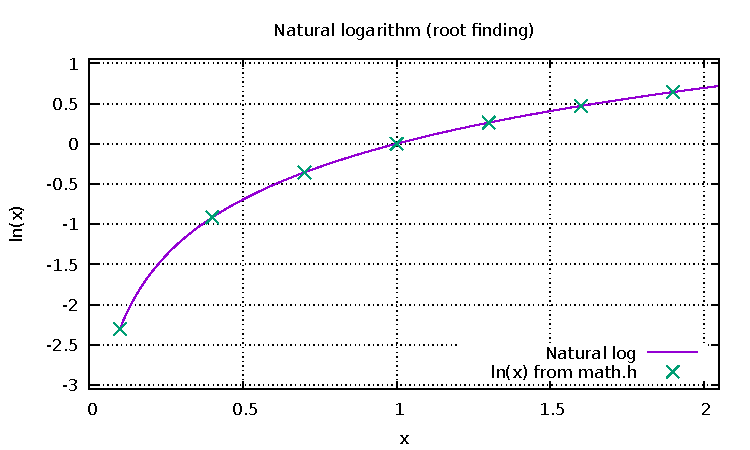
\includegraphics{plot.pdf}
\caption{In the plot one see the natural log found in the exercise as the purple line, while the natural log from math.h is plotted as the crosses.}
\label{fig:nat_log}
\end{figure}

\end{document}


